\section{Evaluation}
\label{sec:evaluation}

We evaluate \eps along four axes: the token-level focus claim
introduced in \S\ref{subsec:token-focus}, qualitative scenarios that
surface specific failure modes, a multi-model calibration benchmark,
and a precision/recall sweep on a 200-entry combined set. The review
loop results follow in \S\ref{subsec:review-loop}.

\subsection{Token-level focus across models and prompt categories}
\label{subsec:token-eval}

Table~\ref{tab:token-focus} (in \S\ref{subsec:token-focus}) reports
the headline token-level numbers. We repeat the structure here with
the per-model breakdown to show that the $\sim 10\%$-flag pattern is
consistent across all four models, not a GPT-4o artefact. The entries
are drawn from \texttt{analyze\_token\_focus.py} run on the
calibration benchmark ($144$ entries: $104$ \textsc{high}, $40$
\textsc{low}, four models).

\begin{table}[h]
\centering
\small
\begin{tabular}{l r r r}
\toprule
\textbf{Model} & \textbf{Fn-flag rate} & \textbf{Tokens $>0.30$}
 & \textbf{Avg fn size} \\
\midrule
\multicolumn{4}{l}{\textsc{high} prompts ($n=104$ across models)} \\
\midrule
GPT-4o        & $96\%$ & $9.8\%$  & $97$ tok \\
GPT-4o-mini   & $95\%$ & $10.2\%$ & $99$ tok \\
GPT-4-turbo   & $97\%$ & $11.1\%$ & $96$ tok \\
DeepSeek V3   & $99\%$ & $11.0\%$ & $102$ tok \\
\addlinespace
\textbf{aggregate} & $\mathbf{97.1\%}$ & $\mathbf{10.5\%}$
   & $\mathbf{98}$ tok \\
\midrule
\multicolumn{4}{l}{\textsc{low} prompts ($n=40$ across models)} \\
\midrule
GPT-4o        & $90\%$  & $12.6\%$ & $78$ tok \\
GPT-4o-mini   & $80\%$  & $12.4\%$ & $76$ tok \\
GPT-4-turbo   & $90\%$  & $13.5\%$ & $82$ tok \\
DeepSeek V3   & $100\%$ & $13.8\%$ & $80$ tok \\
\addlinespace
\textbf{aggregate} & $\mathbf{90.0\%}$ & $\mathbf{13.1\%}$
   & $\mathbf{79}$ tok \\
\bottomrule
\end{tabular}
\caption{Function-level flag rate vs.\ token-level focus, broken out
by model and prompt category. The function-level rate saturates; the
token-level rate is stable at $\sim 10\%$ (flag) across models and
across \textsc{high}/\textsc{low} categories, which means the
localization property holds whether the function-level fire is a
true Type 2 flag or a Type 3 false-positive floor. Per-model counts
have $n=20$--$30$ entries each; numbers are rounded.}
\label{tab:token-focus-per-model}
\end{table}

The aggregate numbers are: $10.4$ tokens per flagged function at the
flag threshold ($10.5\%$ of an average $\sim 98$-token function). The
token review burden reduction relative to reading the whole function
is $89\%$ at the flag threshold.
Figure~\ref{fig:token-focus-detail} (in \S\ref{subsec:token-focus})
shows the per-token trajectory on one representative function;
Figure~\ref{fig:token-focus-teaser} (in \S\ref{sec:introduction})
shows the heat-strip view.

\subsection{Qualitative scenarios}
\label{subsec:scenarios}

Five scenarios exercise distinct failure modes. Scenarios A--D are
single-run and cover four models (GPT-4o-2024-08-06, GPT-4o-mini,
GPT-4-turbo, DeepSeek V3) with \texttt{logprobs=True,
top\_logprobs=5}, temperature $= 0$, and a system prompt specifying
concise naming conventions. Scenario E is evaluated on GPT-4o across
$16$ independent runs to characterize within-model variation;
single-run results for all four models on the other scenarios are in
the multi-model table below.

\begin{table}[h]
\centering
\small
\begin{tabular}{llcccc}
\toprule
 & & \multicolumn{4}{c}{$\eps$ (tier)} \\
\cmidrule(lr){3-6}
 & Scenario & GPT-4o & GPT-4o-mini & GPT-4-turbo & DeepSeek V3 \\
\midrule
A & Stripe deprecation        & $0.878$ \textsc{f} & $0.665$ \textsc{f} & $0.680$ \textsc{f} & $0.775$ \textsc{f} \\
B & OpenAI SDK v0 vs v1       & $0.560$ \textsc{f} & $0.487$ \textsc{f} & $0.678$ \textsc{f} & $0.646$ \textsc{f} \\
C & SQLAlchemy 1.x vs 2.0     & $0.907$ \textsc{f} & $\mathbf{0.000}$ \textsc{c} & $0.911$ \textsc{f} & $0.925$ \textsc{f} \\
D & FastAPI async/sync        & $0.505$ \textsc{f} & $0.506$ \textsc{f} & $0.774$ \textsc{f} & $0.679$ \textsc{f} \\
\bottomrule
\end{tabular}
\caption{Scenarios A--D across four models. \textsc{f} =
\textsc{flagged} ($0.30 \le \eps < 0.95$); \textsc{c} =
\textsc{complete} ($\eps < 0.30$). $15$ of $16$ cells are
\textsc{flagged}; the lone miss is GPT-4o-mini on SQLAlchemy, where
the model committed to one version with no hesitation ($\eps =
0.000$) --- a genuine false negative. No \textsc{high} prompt
crossed the \textsc{paused} threshold ($\eps \ge 0.95$) in this
sweep.}
\label{tab:scenarios-multimodel}
\end{table}

\paragraph{A --- Deprecated API (Stripe).}
\textit{``Charge a customer's card for \$50.''} GPT-4o: $\eps =
0.878$, \textsc{flagged}. The peak token is the method selector
after \texttt{stripe}: \texttt{.Ch} (\texttt{Charge}, prob.\ $0.52$)
vs.\ \texttt{.Payment} (\texttt{PaymentIntent}, prob.\ $0.47$). Both
paths are in the training data; neither is definitively preferred.
All four models flag. The within-function review surface localizes
to the method-selector region rather than the full $98$-token body.

\paragraph{B --- Confident wrongness (OpenAI SDK).}
\textit{``Call GPT-4 and return the response text.''} GPT-4o: $\eps
= 0.560$, \textsc{flagged}. The model generated v0
(\texttt{openai.ChatCompletion.create(\ldots)}) confidently; v0
raises \texttt{AttributeError} on SDK $\ge 1.0$. \eps fired not on
the API call --- the model was certain at that token --- but on
surrounding parameter design. \textsc{flagged} routes the function
to the review loop; the reviewer, examining the full function,
surfaces the deprecated call. This is indirect detection: \eps
flagged adjacent uncertainty, not the failing token itself. All
four models flag.

\paragraph{C --- Syntax split (SQLAlchemy).}
\textit{``Query all active users.''} GPT-4o: $\eps = 0.907$,
\textsc{flagged}, near the top of the \textsc{flagged} range.
GPT-4-turbo and DeepSeek V3 produce similarly high \eps ($0.911$,
$0.925$). GPT-4o-mini, however, produces $\eps = 0.000$
(\textsc{complete}): it commits to one version with no visible
hesitation. This is not a typo or a data-collection artefact; it is
real measured behaviour, and it is a genuine false negative.
GPT-4o-mini committed to one SQLAlchemy version with complete
confidence --- no probability mass on the alternative --- which
means \eps has nothing to observe regardless of whether the chosen
branch is correct. The cross-model contrast is the interesting
finding: intra-generational signal exists only when the model itself
is uncertain, and training-data convergence on one branch silently
removes it. This is the ``confident wrongness'' limitation of
\S\ref{subsec:limitations} made empirically concrete: \eps cannot
detect a model whose prior has converged on a particular API, no
matter which branch the prior points to.

\paragraph{D --- Compatibility mismatch (FastAPI async/sync).}
\textit{``FastAPI endpoint that fetches weather from an external
API.''} GPT-4o: $\eps = 0.505$, \textsc{flagged} (solidly mid-range);
GPT-4-turbo is highest at $0.774$. The model generated
\texttt{async def} with \texttt{requests.get()} inside --- two
individually defensible decisions that combine into a silent bug
(blocks the event loop). The cross-decision mismatch is not
directly what \eps measures: \eps sees token-level uncertainty,
which in this scenario fires on surrounding choices rather than on
the async/sync combination itself. The practical outcome is
unchanged: the function is \textsc{flagged} and reaches the reviewer.

\paragraph{E --- Multi-function module.}
Six auth functions with four interdependent decisions (password
hash, JWT, SQLAlchemy, datetime). \textsc{flagged} on all $16$
runs, $\eps \in [0.69, 0.92]$. Library choices varied across runs
(passlib, bcrypt, PyJWT, python-jose, mixed), but each run looked
internally confident. Early functions $\eps = 0.40$--$0.58$; later
functions frequently $\eps = 0.000$ --- an \emph{uncertainty
collapse} after initial commitment. The first function is the
high-risk window.

\begin{figure}[H]
\centering
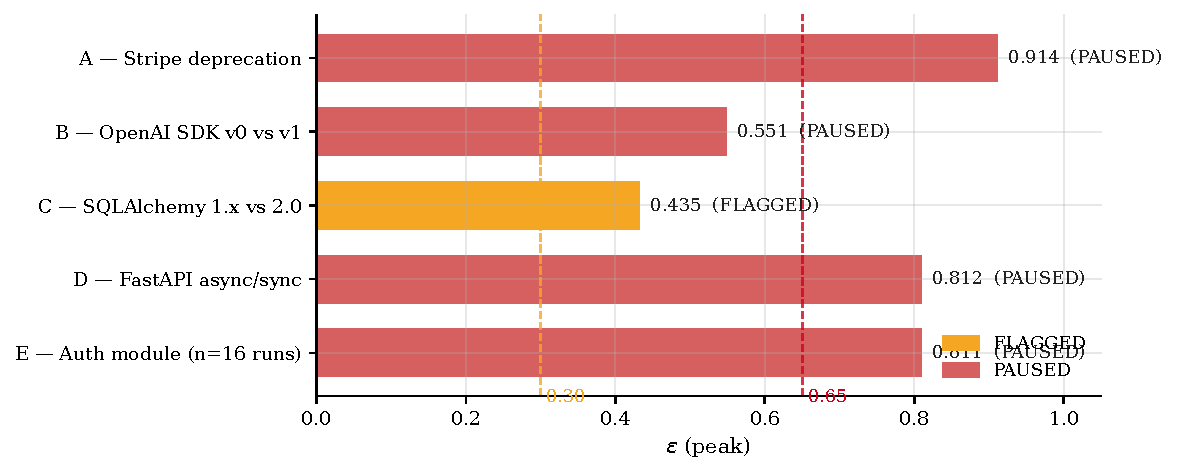
\includegraphics[width=0.85\textwidth]{figures/fig3_scenarios.pdf}
\caption{Scenarios A--E (GPT-4o) summarised by failure class and
peak $\eps$. All five clear the \textsc{flagged} threshold; none
crosses the \textsc{paused} threshold ($\eps \ge 0.95$).}
\label{fig:scenarios}
\end{figure}

\subsection{Scenario E limitation: joint-prompt uncertainty collapse}
\label{subsec:scenarioE}

Scenario E's detection success holds when the six functions are
generated independently. When generated in a \emph{single} prompt
with ``use a consistent library,'' \eps collapses across all six
functions --- not just the later ones. The joint signature list plus
the consistency instruction resolves the library choice before
decoding starts, leaving nothing for \eps to observe
(Table~\ref{tab:scenarioE}, GPT-4o-mini). The practical mitigation
is to generate functions independently; the consistency constraint
can be applied at review time rather than at generation time.

GPT-4o is absent from Table~\ref{tab:scenarioE} because on the
combined-prompt variant it generates additional helper functions
between the six expected signatures, making the positional chunk-%
to-function alignment used for per-function $\eps$ extraction
unreliable. The 16-run variability study uses GPT-4o on
independently-generated functions where alignment is not an issue;
the collapse comparison uses GPT-4o-mini and DeepSeek V3, both of
which produce the six expected functions without interstitial
helpers.

\begin{table}[h]
\centering
\small
\begin{tabular}{l rr rr}
\toprule
 & \multicolumn{2}{c}{GPT-4o-mini} & \multicolumn{2}{c}{DeepSeek V3} \\
\cmidrule(lr){2-3}\cmidrule(lr){4-5}
Function & Combined & Per-fn & Combined & Per-fn \\
\midrule
\texttt{register\_user}          & $0.579$ & $0.627$ & $0.424$ & $0.864$ \\
\texttt{login}                   & $0.820$ & $0.872$ & $0.518$ & $0.972$ \\
\texttt{verify\_token}           & $0.606$ & $0.911$ & $0.372$ & $0.735$ \\
\texttt{refresh\_token}          & $0.414$ & $0.711$ & $0.503$ & $0.957$ \\
\texttt{request\_password\_reset}& $\mathbf{0.295}$ & $0.788$ & $0.764$ & $0.760$ \\
\texttt{reset\_password}         & $0.394$ & $0.728$ & $0.419$ & $0.878$ \\
\bottomrule
\end{tabular}
\caption{Combined generation reduces per-function \eps in both
models. GPT-4o-mini's \texttt{request\_password\_reset} drops below
the \textsc{flagged} threshold ($\mathbf{0.295}$, \textsc{complete});
DeepSeek V3 combined values stay above $0.30$ but are uniformly
lower than per-function values. When context resolves uncertainty
before decoding, there is less for \eps to observe.}
\label{tab:scenarioE}
\end{table}

\begin{figure}[H]
\centering
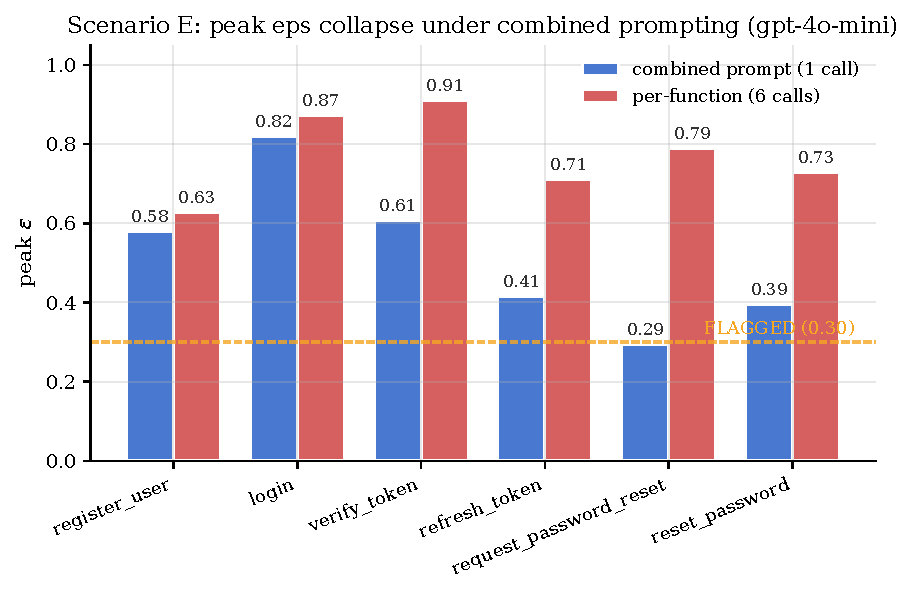
\includegraphics[width=0.85\textwidth]{figures/fig8_scenario_e.pdf}
\caption{GPT-4o-mini: per-function generation keeps all six functions
in the \textsc{flagged} tier; combined generation collapses \eps for
every function, dropping one of six (\texttt{request\_password\_reset},
$\eps = 0.295$) to \textsc{complete}. DeepSeek V3 shows the same
reduction in combined-mode \eps, but all six remain \textsc{flagged}
(Table~\ref{tab:scenarioE}).}
\label{fig:scenarioE}
\end{figure}

\subsection{Multi-model calibration}
\label{subsec:calibration}

Moving from the per-scenario view to aggregate calibration, we
evaluate a 30-prompt set: $10$ \textsc{low} prompts (sort, palindrome,
fibonacci, two-sum --- pure logic) and $20$ \textsc{high} prompts
(API / version-split tasks across Stripe, OpenAI, SQLAlchemy,
FastAPI, Pydantic), run on four models. GPT-4o and DeepSeek V3 both
achieve $85\%$ \textsc{high} detection; GPT-4o-mini and GPT-4-turbo
both achieve $70\%$. DeepSeek V3 carries a higher \textsc{low} FP
rate ($70\%$) than the OpenAI models, consistent with its larger
vocabulary of naming alternatives.

\begin{table}[h]
\centering
\small
\begin{tabular}{lrr}
\toprule
Model & \textsc{high} detection & \textsc{low} FP \\
\midrule
GPT-4o         & $85\%$ (17/20) & $50\%$ (5/10) \\
GPT-4o-mini    & $70\%$ (14/20) & $60\%$ (6/10) \\
GPT-4-turbo    & $70\%$ (14/20) & $60\%$ (6/10) \\
DeepSeek V3    & $85\%$ (17/20) & $70\%$ (7/10) \\
\bottomrule
\end{tabular}
\caption{Calibration at the \textsc{flagged} threshold ($\eps \ge
0.30$). $95\%$ Wilson CIs: $\pm 17$pp \textsc{high}, $\pm 30$pp
\textsc{low}. Three \textsc{high} prompts produce $\eps = 0.000$
across all four models (\texttt{HTTP-GET-to-JSON}, \texttt{Pydantic
serialization}, \texttt{async HTTP GET}) --- \emph{confidently-%
resolved domains} where training priors have converged.}
\label{tab:calibration}
\end{table}

\subsection{\textsc{low} ground truth}
\label{subsec:low-gt}

All $30$ \textsc{low} functions passed \texttt{exec()} assertions.
Tier breakdown: \textsc{complete} $5$, \textsc{flagged} $20$,
\textsc{paused} $5$. The $25$ non-\textsc{complete} fires are all
Type 3 false positives: correct code where \eps observed hesitation
between algorithm structures that are both correct (brute vs.\ hash
two-sum, recursive vs.\ iterative Fibonacci). Per
\S\ref{subsec:types}, these are classified Type 3 precisely because
both alternatives are correct; the decoder state that produced them
is indistinguishable from the Type 2 state that fires on
\texttt{Charge} vs.\ \texttt{PaymentIntent}.

\subsection{Precision/recall at tier boundaries}
\label{subsec:pr}

We now consolidate the calibration numbers into a single precision/
recall view. On a 200-entry combined set ($30$ \textsc{low} exec-%
verified plus $170$ \textsc{high} LLM-judged;
see~\S\ref{subsec:gt-disclosure}), $53$ true failures and $147$
correct:

\begin{table}[h]
\centering
\small
\begin{tabular}{lrrr}
\toprule
Threshold & Precision & Recall & F1 \\
\midrule
$\eps \ge 0.30$ (\textsc{flagged+}) & $0.272$ & $\mathbf{1.000}$ & $0.428$ \\
$\eps \ge 0.95$ (\textsc{paused})   & $\mathbf{0.309}$ & $0.547$ & $0.394$ \\
\bottomrule
\end{tabular}
\caption{$n=200$, $53$ positives; $95\%$ Wilson CI on
\textsc{flagged+} precision $[0.22, 0.33]$. Base failure rate
$26.5\% \approx$ \textsc{flagged+} precision at the function level.
The function-level gate's precision is barely above base rate; its
value is recall, which is what directs the reviewer to the right
functions, combined with the token-level localization of
\S\ref{subsec:token-focus}, which directs the reviewer to the right
tokens within those functions. \textsc{high} ground truth for
$170/200$ entries is LLM-judged by GPT-4o
(\S\ref{subsec:gt-disclosure}); \textsc{low} ground truth ($30/200$)
is \texttt{exec()}-verified.}
\label{tab:pr}
\end{table}

Function-level tiers are urgency signals, not calibrated
probabilities. The useful binary boundary is \textsc{complete} vs.\
\textsc{flagged+}. What actually makes the system work at the
developer's end is that \textsc{flagged+} comes paired with a
token-level attribution (\S\ref{subsec:token-focus}).

\subsection{Review loop: context-free vs.\ context-primed reviewer}
\label{subsec:review-loop}

Having established stage-$1$ recall and token-level localization, we
turn to the stage-$2$ reviewer that converts the recall-maximizing
filter into an end-to-end system with usable precision. The
reviewer is not asked to re-read the function. It is given the
function plus the specific high-\eps tokens, and asked to evaluate
those tokens in context. The token-level attribution is what makes
the reviewer fast: at current API prices, pointing the reviewer at
a handful of tokens rather than $98$ costs fractions of a cent per
entry and completes in seconds.

Evaluated on $201$ entries (production FastAPI codebase plus
scenarios A--E, three models). Every \textsc{flagged+} entry is sent
in parallel to a GPT-4o reviewer returning \textsc{cleared}/\textsc{%
confirmed}; a consolidation pass processes remaining suspects. The
\textbf{context-free} variant uses no reviewer context; the
\textbf{context-primed} variant injects model-specific learned
false-positive patterns from a prior clean run (injecting suspect
patterns caused over-flagging in pilots). All results use GPT-4o as
reviewer; reviewer-model ablation (e.g., with Claude or DeepSeek)
is left to future work.

\begin{table}[h]
\centering
\small
\begin{tabular}{lrr}
\toprule
Metric & Context-free & Context-primed \\
\midrule
Cleared by reviewer        & $107/201$ ($53.2\%$) & $138/201$ ($68.7\%$) \\
Forwarded to consolidation & $89$                 & $57$ \\
Confirmed true failures    & $85$ ($42.3\%$)      & $57$ ($28.4\%$) \\
Late false positives       & $4$                  & $0$ \\
\bottomrule
\end{tabular}
\caption{``Late false positive'' = an entry marked \textsc{confirmed}
that was in fact correct on manual inspection. The context-primed
variant is the preferred production configuration.}
\label{tab:review}
\end{table}

\begin{figure}[H]
\centering
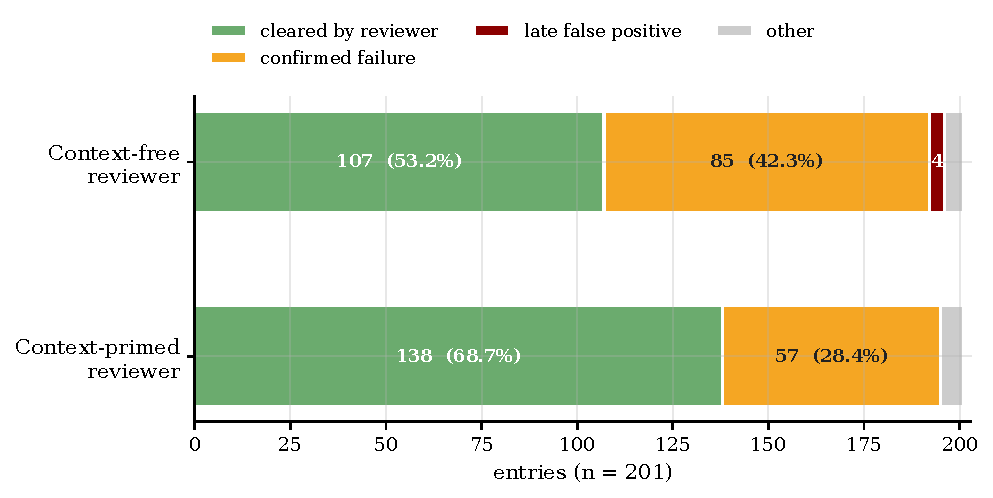
\includegraphics[width=0.85\textwidth]{figures/fig7_review_loop.pdf}
\caption{Injecting learned FP patterns into the reviewer (context-%
primed vs.\ context-free) shifts $31$ additional entries from
consolidation to cleared and eliminates late false positives, at the
cost of suppressing some true failures the context-free reviewer
forwarded.}
\label{fig:review-loop}
\end{figure}

End-to-end failure rates: GPT-4o-mini $40\%$, GPT-4o $29\%$,
DeepSeek V3 $26\%$. Because stage-$1$ recall is $100\%$, end-to-end
precision is determined entirely by the reviewer's precision on the
\textsc{flagged+} set; the reviewer's own precision is in turn
driven by how well it can evaluate the specific tokens the filter
attributes. The context-primed variant's zero late-FP result rests
on $n=57$ confirmed entries and needs a larger validation study.
The stage-$1$ recall guarantee applies to entries that reach the
reviewer; entries the reviewer clears were not independently verified.
